%================================================================
\chapter{O programa E-foto}
%================================================================

Nesse capítulo será apresentado o software E-foto, suas funcionalidades e o que deve ser feito para sua obtenção e instalação. Sendo explicado quais pacotes serão necessários para o funcionamento do programa após a realização do seu download.
%fiz uma introduçaõ genérica, que deve ser modificada quando o projeto for mais completo

\section{O que é o E-foto}
\subsection{O que é e qual o objetivo do E-foto}
De acordo com o website oficial \textit{http://www.efoto.eng.uerj.br/about-e-foto}, o E-foto é um software livre para fotogrametria digital que é desenvolvido pelo laboratório de fotogrametria da Universidade do Estado do Rio de Janeiro desde 2004 e tem como objetivo, além da criação de um software inteiramente funcional (uma estação fotogramétrica gratuita), levar aos alunos o conhecimento de forma gratuita sobre fotogrametria digital, sendo de forma didática ou até mesmo na prática por meio de acesso ao código, uso da plataforma e até criação de novos módulos para o software.

\subsection{O que é a fotogrametria}
A fotogrametria remete etimologicamente à ideia da realização de medidas em imagens, e tem como objetivo geral a recriação de parte de um espaço tridimensional a partir de imagens bidimensionais obtidas sem contado entre o sensor e o alvo fotografado. A fotogrametria é classificada de acordo com e evolução dos métodos de obtenção e de análise das imagens, cuja realização vai cada vez mais deixando de ser analógica e se tornando digital, aumentando a precisão e a velocidade, e deixando de lado o trabalho mais artesanal e demorado.
Segundo a \textit{American Society for Photogrammetry and Remote Sensing} (ASP, 1980):

\begin{quote}
	``A fotogrametria é a arte, ciência, e tecnologia de obtenção de informações confiáveis sobre os objetos físicos e o meio ambiente através de processos de gravação, medição e interpretação de imagens fotográficas e padrões da energia eletromagnética radiante e outros fenômenos.''
\end{quote}

\subsection{Classificações da fotogrametria}
Usando como referência o  livro \textbf{Fotogrametria Digital}, escrito por Luiz Coelho e Jorge Nunes Brito \cite{bib:livrofotogrametria}, publicado pela Editora da Universidade do Estado do Rio de Janeiro, as classificações da fotogrametria são feitas de maneira histórica. Assim, a \textbf{fotogrametria pioneira} (1840-1900) se deu alguns anos após a invenção da fotografia e com a ideia de usá-la para auxílio na topografia, mas sem grandes resultados, sua utilização começou mesmo a ser difundida em 1851 para documentação de edifícios históricos, sendo criados os seus primeiros métodos de utilização, mas somente com avanços na tecnologia aérea a fotogrametria pôde realmente ser impulsionada e a dificuldade na obtenção de imagens aéreas foi reduzida. 

A \textbf{fotogrametria analógica} (1901-1950) se deu após a primeira revolução da fotogrametria, que ocorre com a invenção do aparelho \textit{estereocomparador} que colocava aparelhos óptico mecânicos no lugar de inúmeros cálculos matemáticos, facilitando a vida dos usuários. Em 1911 foi aumentado o uso de retificadores analógicos devido à criação de um método funcional de retificação de imagens que tornou usual a utilização das fotografias para mapear extensas superfícies. A Alemanha e a Suíça tinham aparelhos que tornavam possíveis a criação de cartas topográficas de alta precisão. Esse avanço na tecnologia da fotogrametria fez com o trabalho se tornasse cada vez mais especializado, assim passou a ter necessidade de um profissional de conhecimento técnico para a realização do mesmo. Paralelamente a esse avanço ocorreram também mais fatos que ajudaram no avanço da fotogrametria em geral, o processo de foto triangulação analógica facilitou o trabalho externo, as câmaras métricas que realizavam impressões de imagens relevantes quanto às coordenadas, o que fez aumentar a precisão das medidas realizadas.

A partir da evolução da tecnologia computacional, grande parte do trabalho manual e mecânico foram substituídos por tarefas feitas diretas no computador dando início a era da fotogrametria analítica (1951-1990). Com o auxílio da computação os cálculos em cima das imagens eram feitos pelos computadores e passou a ter a possibilidade da utilização de conjunto de imagens para serem medidas simultaneamente assim como um estudo mais completo da propagação de erros, passou a ser permitido também a utilização de câmeras não-métricas.
Com o avanço tecnológico ocorreram mudanças bem significativas no quesito de obtenção de imagens uma vez que com a criação das câmeras digitais ou até mesmo com a utilização de um escâner se pôde obter imagens digitais e com avanços da computação os computadores passaram a processar essas imagens, com isso surgiu a era da fotogrametria digital (1990-atualmente). Para o processo foram criadas estações com aparelhos específicos para a fotogrametria, as chamadas estações fotogramétricas digitais onde todo o processo é feito por meio de computadores desde a sua entrada (fotos digitais ou analógicas escaneadas) até a sua saída (dados digitais compatíveis com softwares existentes).

\subsection{Obtenção de imagens fotogramétricas digitais}
Podemos obter uma imagem fotogramétrica digital de duas maneiras: por meio de escâneres (digitalização de imagens obtidas analogicamente) e por meio de câmeras fotogramétricas digitais (maneira mais direta). Com a utilização dos escâneres normalmente é possível por meio de um software obter a melhor configuração para a digitalização desejada, mas mesmo com essa configuração existe a ocorrência de perda de alguma informação durante o processo de digitalização já que os dispositivos não possuem capacidade de digitalizar toda a complexidade da imagem. Essa responsabilidade de configurar os escâneres e seus respectivos programas para que a perda seja menor possível de maneira que a imagem ainda possa ser utilizada e mantendo a integridade da imagem original é humana, do profissional da área fotogramétrica. No caso do uso das câmeras fotogramétricas digitais ainda existe muita limitação para seu uso, pois possuem um preço muito elevado. Ainda podem ocorrer problemas na obtenção das imagens devido ao formato das lentes das câmeras, o que também deve ser tratado para manter a integridade de uma imagem fotogramétrica digital.

\subsection{Importância e os problemas da fotogrametria digital}
A importância da fotogrametria digital é justamente manter o avanço das ferramentas utilizadas para a fotogrametria condizente com os avanços tecnológicos, assim cada vez mais os processos ficam computadorizados e consequentemente mais rápidos e automatizados.

Apesar da tendência a automatizar todo o processo da fotogrametria proposto ideologicamente pela fotogrametria digital ainda existe o problema de que as superfícies são muito imperfeitas e possuem inúmeras descontinuidades que dificultam bastante a obtenção de valores razoáveis automaticamente mapeados então a participação humana se faz necessária mesmo que só para supervisionar a qualidade do que está sendo mapeado, tornando o trabalho semiautomático ou o mais automático possível tentando não comprometer a qualidade do processo.


\section{Utilização do E-foto}

A importância do E-foto e suas vantagens vêm desde a sua criação, pois a mesma promove um encontro entre campos diferentes da engenharia e suas especialidades, sendo eles a engenharia de computação e a engenharia cartográfica, gerando assim um conhecimento mesmo que básico do que pode ser feito em uma área que não é a necessariamente a especialidade do aluno ou usuário. Outra vantagem vem da possibilidade de colocar em prática determinados assuntos que são vistos de forma teórica em sala de aula ou em livros em ambas as vertentes da engenharia, o que por muitas vezes não é feito durante a graduação e quando é feito, raramente é com algo de tamanha importância quanto o E-foto, que é uma estação fotogramétrica digital que tem acesso público, então a qualidade da sua criação tem grande impacto em sua utilização, e essa qualidade é exigida pelos professores criadores já que os mesmos prezam bastante por essa qualidade, assim como a instituição de ensino como um todo.

Fazer parte do projeto E-foto é uma rara oportunidade de aprender fotogrametria e programação na prática, seja na sua criação, nos testes feitos ou na própria utilização, já que oportunidades como essa são difíceis. E com o avanço tecnológico que fez com que a maioria dos dados cartográficos fosse feita por esse tipo de tecnologia que é a fotogrametria digital, ter um software livre e gratuito disponível para isso faz do E-foto um projeto diferenciado e muito importante.


\section{Instalação do E-foto}
\subsection{Em Sistemas Linux}
% instalação usando o .deb disponibilizado pelo site.
Nessa parte o usuário irá instalar o E-foto através do download e instalação a partir do arquivo .deb e para isso será necessário que ele acesse o web site:
\url{http://www.efoto.eng.uerj.br/download/latest-version}
 e realize o download da opção designada para Ubuntu na aba latest version.
%detalhes, detalhes. Capture telas, coloque as imagens aqui. explique passo a passo. Ainda está muito genérico.
\subsection{Em Sistemas Windows}
% instalação usando o .msi disponibilizado pelo site
\subsubsection{Passo 1 - Baixar o instalador do website}
Nessa parte o usuário irá instalar o E-foto através do download e instalação a partir do arquivo .msi e para isso será necessário que ele acesse o web site \url{http://www.efoto.eng.uerj.br/download/latest-version} e realize o download da opção designada para Windows na aba latest version como é mostrado na Figura \ref{fig:downmsi}.

\begin{figure}[!ht]{17cm}
	\centering
	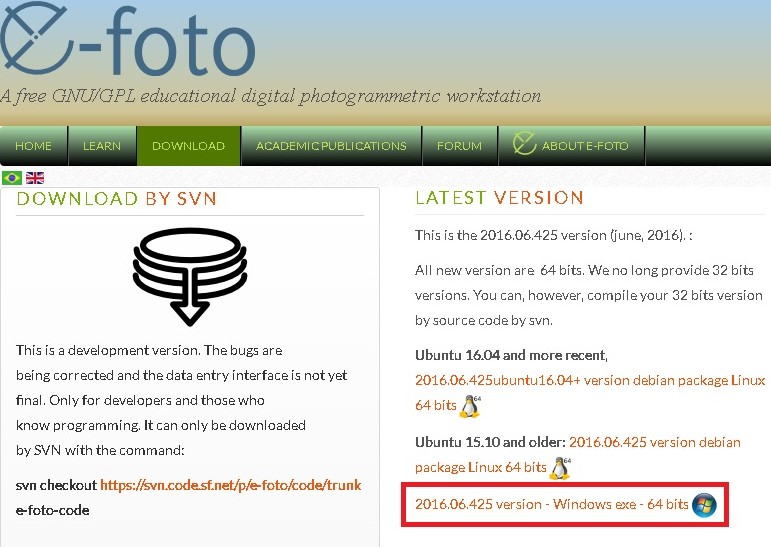
\includegraphics[width=8cm]{Figuras/downmsi.jpg}
	\caption{Realizando download do instalador do E-foto} \label{fig:downmsi}
\end{figure}

\subsubsection{Passo 2 - Realizar a instalação}
Normalmente o arquivo baixado vai para a pasta Downloads do computador do usuário e para realizar a instalação basta dar um clique duplo nesse arquivo, clicar na opção Next, ler e aceitar os termos do contrato e clicar novamente em Next, no próximo passo o usuário deve escolher o caminho onde o E-foto será instalado e depois o usuário deve clicar em Install e a instalação será realizada automaticamente conforme a figura \ref{fig:installmsi}.
 
\begin{figure}[!ht]{17cm}
   \centering
   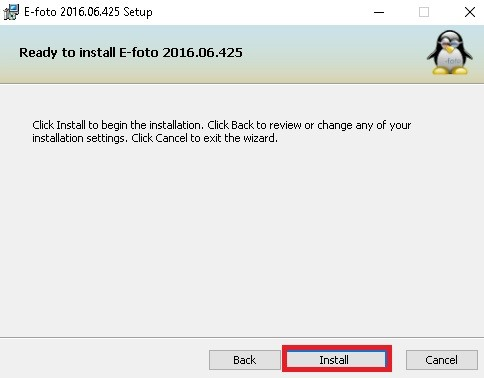
\includegraphics[width=8cm]{Figuras/installmsi.jpg}
   \caption{Instalando E-foto através do instalador} \label{fig:installmsi}
\end{figure}
  
\subsubsection{Passo 3 - Executar o programa E-foto}
Após a instalação terminar, basta manter a opção launch E-foto e clicar na opção Finish, como mostra a figura \ref{fig:launch1} que o E-foto será executado, ou fechar o instalador e buscar o E-foto nos seus aplicativos instalados conforme a figura \ref{fig:launch2}. Neste formato o instalador do E-foto instalará tudo o que é necessário para o funcionamento sem a necessidade de configurações adicionais.

\begin{figure}[!ht]{17cm}
	\centering
	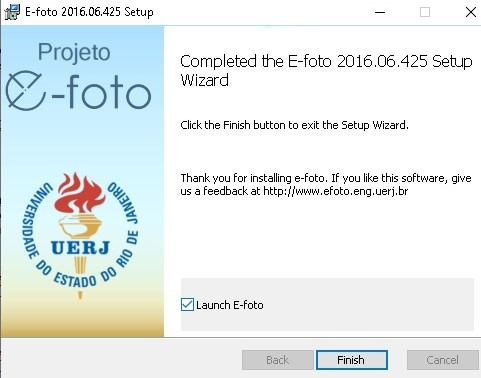
\includegraphics[width=8cm]{Figuras/launch1.jpg}
	\caption{Executando o E-foto pelo instalador} \label{fig:launch1}
\end{figure}

\begin{figure}[!ht]{17cm}
	\centering
	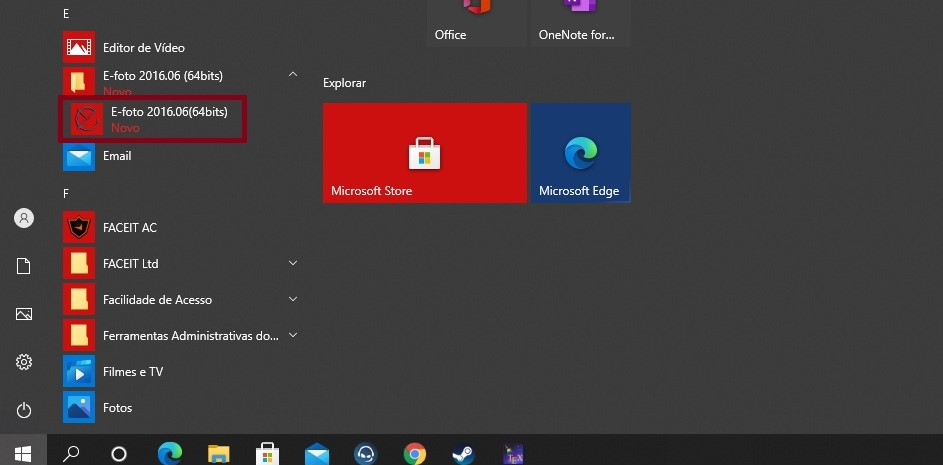
\includegraphics[width=8cm]{Figuras/launch2.jpg}
	\caption{Buscando E-foto nos aplicativos} \label{fig:launch2}
\end{figure}



\subsection{Compilação do E-foto a partir dos fontes}
\subsection{Em Sistemas Linux}

\subsubsection{Passo 1 - Baixar código fonte}
Primeiramente, para realizar a instalação do software E-foto, o usuário deve fazer o download do seu código fonte e para isso é necessário a instalação do subversion, se já não estiver instalado. Para tal, o usuário deve abrir o terminal do seu sistema Linux, que pode ser feito digitando terminal na barra de busca ao apertar a tecla do Windows no seu teclado ou pelo atalho do teclado \texttt{ctrl + alt + T}. Com o terminal aberto, o usuário começará a instalação do SVN com os comandos: 
\begin{lstlisting}[language=bash]
	$ sudo apt update
	$ sudo apt install subversion
\end{lstlisting}

Com o SVN instalado e configurado, basta o usuário digitar no terminal o comando:
\begin{lstlisting}[language=bash]
 $ svn checkout https://svn.code.sf.net/p/e-foto/code
\end{lstlisting}

Com a utilização desse comando o download de todo o código fonte do software E-foto será feito automaticamente.  
    
\subsubsection{Passo 2 - Instalar pacotes necessários à compilação}  
Após a realização do download do código fonte do E-foto, o usuário deve ficar atento aos pacotes necessários em seu ambiente para que o software E-foto possa ser instalado e ter seu funcionamento sem erros. Para a instalação dos pacotes o usuário deve buscar abrir novamente o terminal. Os pacotes necessários para instalação do e-foto são:
\begin{itemize}
   	\item libgdal.dev
   	\item build-essential
   	\item libfontconfig1
   	\item mesa-common-dev
   	\item libx11-xcb-dev
   	\item libglu1-mesa-dev
\end{itemize}
Cada pacote deve ser instalado com respectivamente com os seguintes comandos:	
\begin{lstlisting}[language=bash]
	$ sudo apt install libgdal-dev
	$ sudo apt install build-essential
	$ sudo apt install libfontconfig1
	$ sudo apt install mesa-common-dev
	$ sudo apt install libx11-xcb-dev 
	$ sudo apt install libglu1-mesa-dev
\end{lstlisting}				
	
O pacote libgdal.dev é o contém as funcionalidades da GDAL, onde GDAL é uma biblioteca de tradução para formatos geoespaciais. O pacote libfontconfig1 contém uma biblioteca projetada para achar fontes no sistema e selecioná-las de acordo com os requisitos especificados pelas aplicações, e o usuário deve instalar o driver XCB e o OpenGl através dos pacotes mesa-common-dev, libx11-xcb-dev e libglu1-mesa-dev. 
    
\subsection{Passo 3 - Instalar os pacotes de instalação do Qt 5}   
A instalação do Qt 5 via terminal deve ser feita através dos seguintes pacotes:
\begin{itemize}
	\item qt5-default
	\item qt5-qmake
\end{itemize}   
Esses pacotes devem ser instalados através dos seguintes comandos do terminal:
\begin{lstlisting}[language=bash]
	$ sudo apt install qt5-default
	$ sudo apt install -y qt5-qmake
\end{lstlisting}	
    
Após esses procedimentos o usuário ja terá um ambiente de compilação pronto para a instalação do E-foto, assim como o plataforma em que o mesmo foi desenvolvido.
    
\subsection{Passo 4 - Compilar e executar o software E-foto}
Para compilar e executar o código do E-foto via terminal, após a realização de todos os passos necessários, o usuário deve utilizar os seguintes comandos no terminal:
\begin{lstlisting}[language=bash]
   	$ cd diretório/
   	$ qmake e-foto.pro
   	$ make
   	$ ./build/bin/e-foto
\end{lstlisting}
   
O comando \textit{cd diretório/} servirá para o usuário percorrer o caminho até o diretório onde está o arquivo e-foto.pro (atualmente \textit{code/branches/e-foto-trunk-candidate}), depois o qmake e o make irão realizar a compilação e gerar o executável do E-foto. Por fim o último comando irá executar o software E-foto.

\subsection{Em Sistemas Windows}

\subsubsection{Passo 1 - Baixar código fonte}
 Para começara instalação do E-foto em sistemas Windows, o usuário deve realizar o download do código fonte do E-foto e para isso o melhor caminho é ulilizar o subversion, que no Windows pode ser feito através de um programa chamado TortoiseSVN que pode ser baixado gratuitamente por esse link https://tortoisesvn.net/downloads.html na opção mostrada na figura \ref{fig:tortoise}, após a instalação do TortoiseSVN, o usuário deve buscar no programa a opção de SVN Checkout, que pode ser encontrada ao clicar o botão direito do mouse na área de trabalho conforme é mostrado na figura \ref{fig:checkout} e no espaço para colar uma URL (primeira opção disponível) colocar https://svn.code.sf.net/p/e-foto/code como é visto na figura \ref{fig:url}, que deve gerar o download de todo o código fonte do E-foto.
 
 \begin{figure}[!ht]{17cm}
 	\centering
 	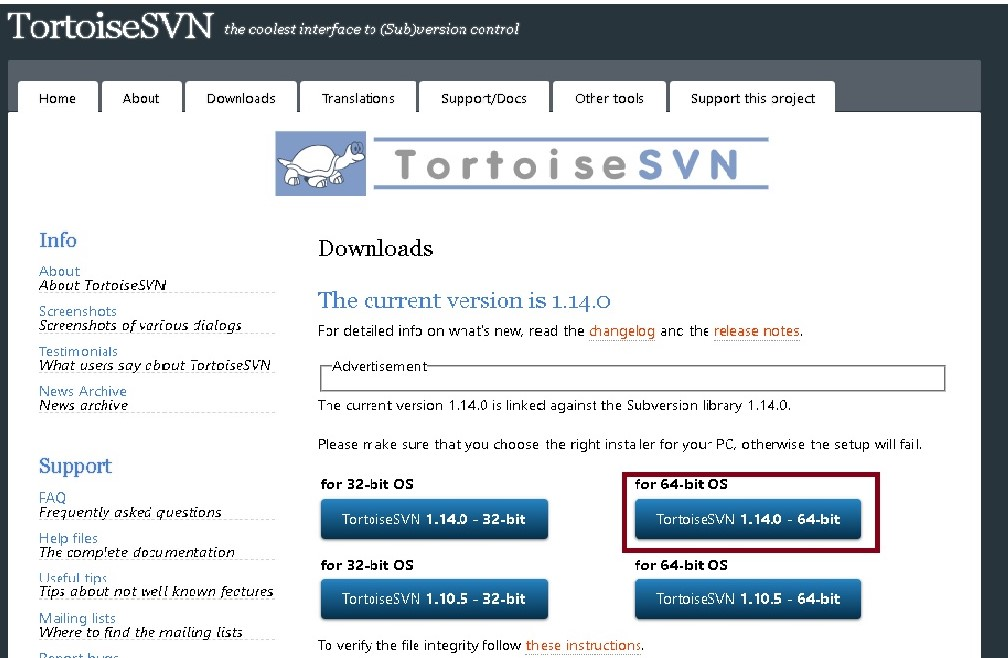
\includegraphics[width=8cm]{Figuras/tortoise.jpg}
 	\caption{Download do TortoiseSVN} \label{fig:tortoise}
 \end{figure}

\begin{figure}[!ht]{17cm}
	\centering
	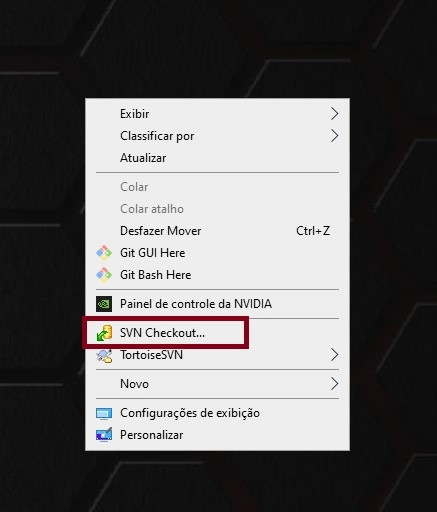
\includegraphics[width=8cm]{Figuras/checkout.jpg}
	\caption{Buscando a opção de checkout} \label{fig:checkout}
\end{figure}

\begin{figure}[!ht]{17cm}
	\centering
	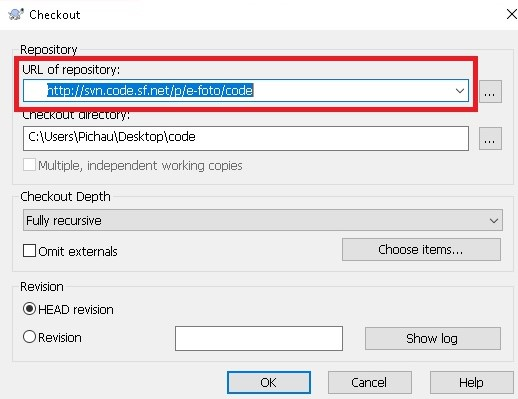
\includegraphics[width=8cm]{Figuras/url.jpg}
	\caption{Realizando o download com a URL} \label{fig:url}
\end{figure}
 
\subsubsection{Passo 2 - Download dos pacotes binários da Gdal no Windows} 
 O próximo passo é o download dos pacotes binários do Gdal no Windows que pode ser realizado através desse link https://repo.msys2.org/distrib/x86\_64/msys2-x86\_64-20200720.exe, que realizará o download do MSYS, após a conclusão do download e da instalação do MSYS (que deve ser feita no drive C, que normalmente é o default) o usuário deve executar mSYS, o que vai abrir o terminal do próprio MSYS que contém uma versão portada do gerenciador de pacotes Pacman conforme pode ser visto na figura \ref{fig:terminalgdal}, nessa última versão do Pacman deve ser digitado no terminal o comando:
 
 \begin{figure}[!ht]{17cm}
 	\centering
 	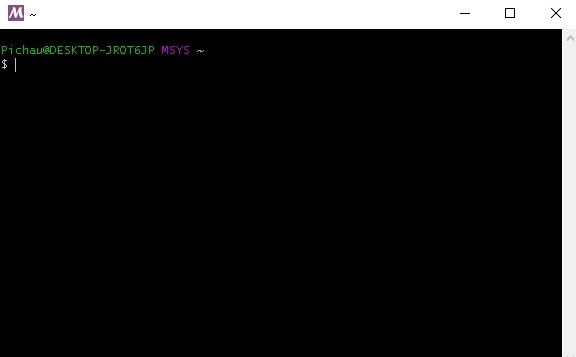
\includegraphics[width=8cm]{Figuras/terminalgdal.jpg}
 	\caption{Terminal MSYS} \label{fig:terminalgdal}
 \end{figure}
 
 \begin{lstlisting}[language=bash]
 	$ pacman -Syuu
 \end{lstlisting}

 Esse comando irá gerar uma série de instruções a serem seguidas até que o usuário possa repetir o comando e receber a mensagem de que nada necessita ser atualizado. Com o ambiente atualizado, o usuário deve digitar o seguinte comando:
  \begin{lstlisting}[language=bash]
 	$ pacman -S mingw64/mingw-w64-x86\_64-gdal
 	$ gdalinfo --version
 \end{lstlisting}

 Esses comandos que realizarão finalmente o download e instalação dos pacotes binários da GDAL e dirão qual versão que foi instalado, respectivamente. 
 
 \subsubsection{Passo 3 - Baixar e configurar o Qt 5 e o Qt Creator}
 Nessa etapa o usuário deve realizar o download do Qt 5 e do Qtcreator no website https://www.qt.io/download como mostrado na figura \ref{fig:downqt} , deixando claro que na parte da instalação deve ser escolhido para instalar apenas as opções do mingw 64-bits, e o Qt 5 referente a esse sistema que é visto na figura \ref{fig:qtinstallconfig}. Com os arquivos do código fonte do E-foto disponíveis o usuário deve procurar no caminho e-foto-code/branches/e-foto-trunk-candidate por um arquivo chamado e-foto.pro mostrado na figura \ref{fig:openpro}. Quando abrir o projeto no Qtcreator será necessário configurar o que deverá ser usado, começando pela escolha do kit que será usado que devem ser os mesmos escolhidos na instalação do Qt 5, ou seja, o mingw 64-bits e a versão do Qt referente a esse sistema como mostra a figura \ref{fig:qtkit}. Após o projeto estar aberto, o usuário deve ir na guia project e desmarcar a opção shadow build, e depois procurar na aba build a opção build E-foto, quando acabar a compilação é só clicar na opção Run que também pode ser encontrado na aba build e o E-foto vai abrir pronto para o uso como estão assinalados na figura \ref{fig:projectbuild}.
 %coloque capturas de tela aqui. Aliás, como o processo é gráfico, sempre use capturas de telas e não simplesmente texto.
  \begin{figure}[!ht]{17cm}
  	\centering
 	
\includegraphics[width=8cm]{Figuras/downqt.jpg}
 	\caption{Download do Qt 5 pelo website} \label{fig:downqt}
 \end{figure}

 \begin{figure}[!ht]{17cm}
 	\centering
	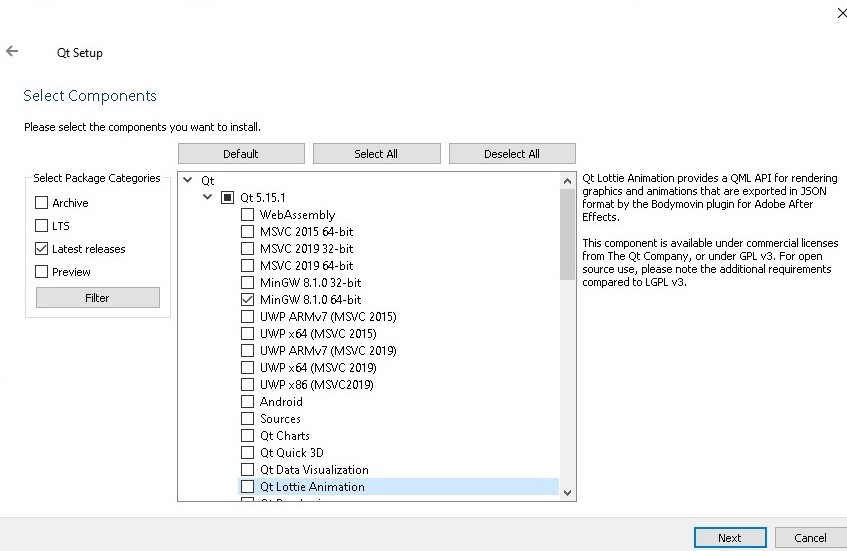
\includegraphics[width=8cm]{Figuras/qtinstallconfig.jpg}
	\caption{configuração da  instalação do Qt 5} \label{fig:qtinstallconfig}
\end{figure}

 \begin{figure}[!ht]{17cm}
 	\centering
	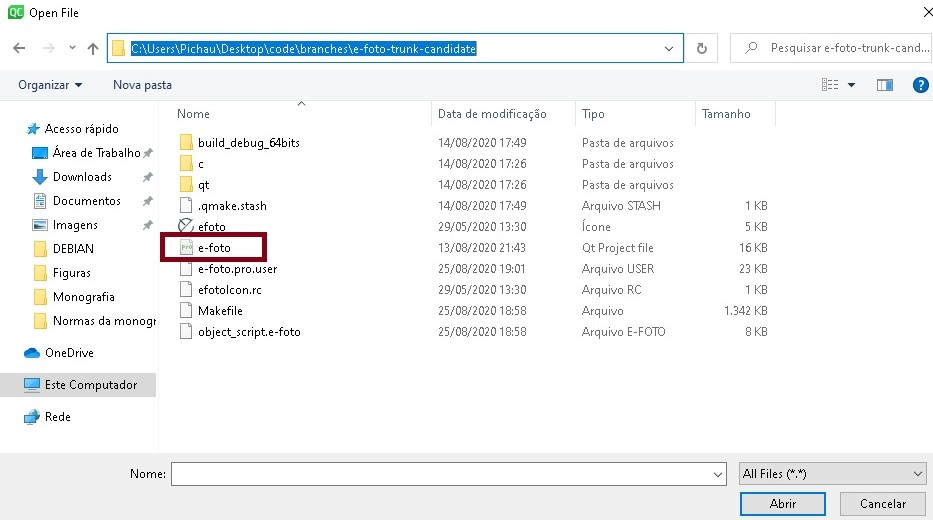
\includegraphics[width=8cm]{Figuras/openpro.jpg}
	\caption{Caminho do arquivo do projeto E-foto} \label{fig:openpro}
\end{figure}

 \begin{figure}[!ht]{17cm}
 	\centering
	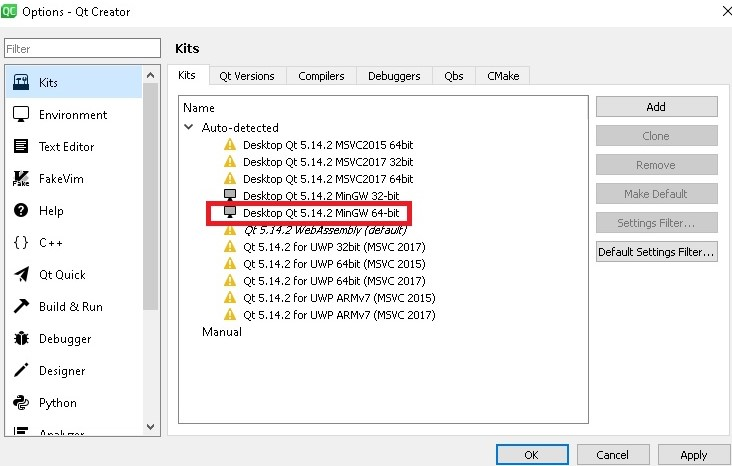
\includegraphics[width=8cm]{Figuras/qtkit.jpg}
	\caption{Configuração do kit} \label{fig:qtkit}
\end{figure}

 \begin{figure}[!ht]{17cm}
 	\centering
	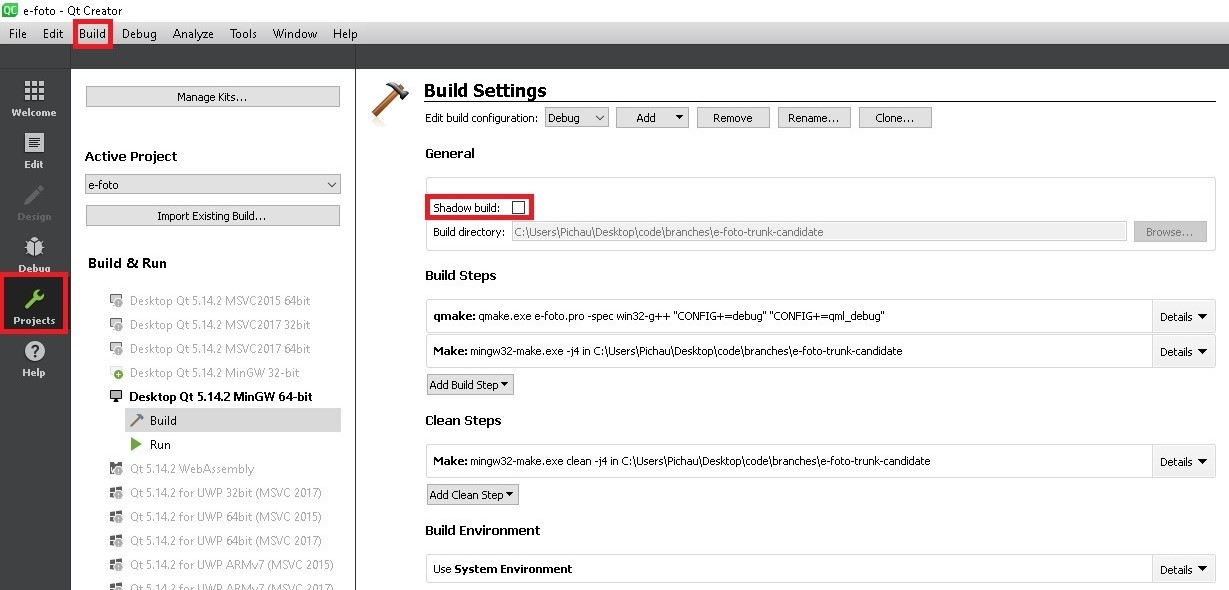
\includegraphics[width=8cm]{Figuras/projectbuild.jpg}
	\caption{Locais buscados para a compilação} \label{fig:projectbuild}
\end{figure}
 